\documentclass{amsart}

% \usepackage[notref,notcite]{showkeys}
\usepackage[style=authoryear,ibidtracker=false,uniquename=false,giveninits=true,terseinits=true,maxbibnames=5,backend=biber]{biblatex}
\usepackage{float}
\usepackage{graphicx}

\renewbibmacro{in:}{}
\addbibresource{rnni_polynomial.bib}

\newtheorem{lemma}{Lemma}
\newtheorem{theorem}{Theorem}

\newcommand{\rnni}{\mathrm{RNNI}}
\newcommand{\findpath}{\textsc{FindPath}}
\newcommand{\mrca}{\mathrm{mrca}}
\newcommand{\rank}{\mathrm{rank}}
\newcommand{\nni}{\mathrm{NNI}}

\graphicspath{{figures/}}

\begin{document}


\begin{lemma}
    Let $p = \findpath(T,R)$ be the path from tree $T$ to $R$ that is computed by the $\findpath$ algorithm.
    Let $\hat{T}$ be the tree at the beginning of iteration $i$ of the algorithm in which the most recent common ancestor of cluster $C_i$ is moved down.
    Then there is no tree on $p$ where a cluster $C_j$ of $R$ with $\rank((C_i)_{\hat{T}}) \geq \rank((C_j)_{\hat{T}})$ and $i < j$ has the same most recent common ancestor as $C_i$.
\end{lemma}

\proof

For proving the lemma by contradiction we assume that clusters $C_i, C_j$ exist such that their most recent common ancestors do not coincide in $\hat{T}$, but in some tree following this one on $p$.
Let $T''$ be the first tree where the most recent common ancestors coincide and let $T'$ be the tree on $p$ that is immediately followed by $T''$.
It is obvious that the $\rnni$ between $T'$ and $T''$ is an $\nni$ move.
It is $\rank((C_i)_{T'}) = \rank((C_j)_{T'}) + 1$ and $\rank((C_i)_{T''}) = \rank((C_j)_{T''}) = \rank((C_j)_{T'})$.
Considering the illustration in Figure~\ref{fig:nni_move}, we can follow from the second equality that $C_i, C_j \subseteq A \cup C$, which is contradicting $\rank((C_i)_{T'}) = \rank((C_j)_{T'}) + 1$, as this implies $C_j \cap B \neq \emptyset$ in that figure.


\begin{figure}[H]
\centering
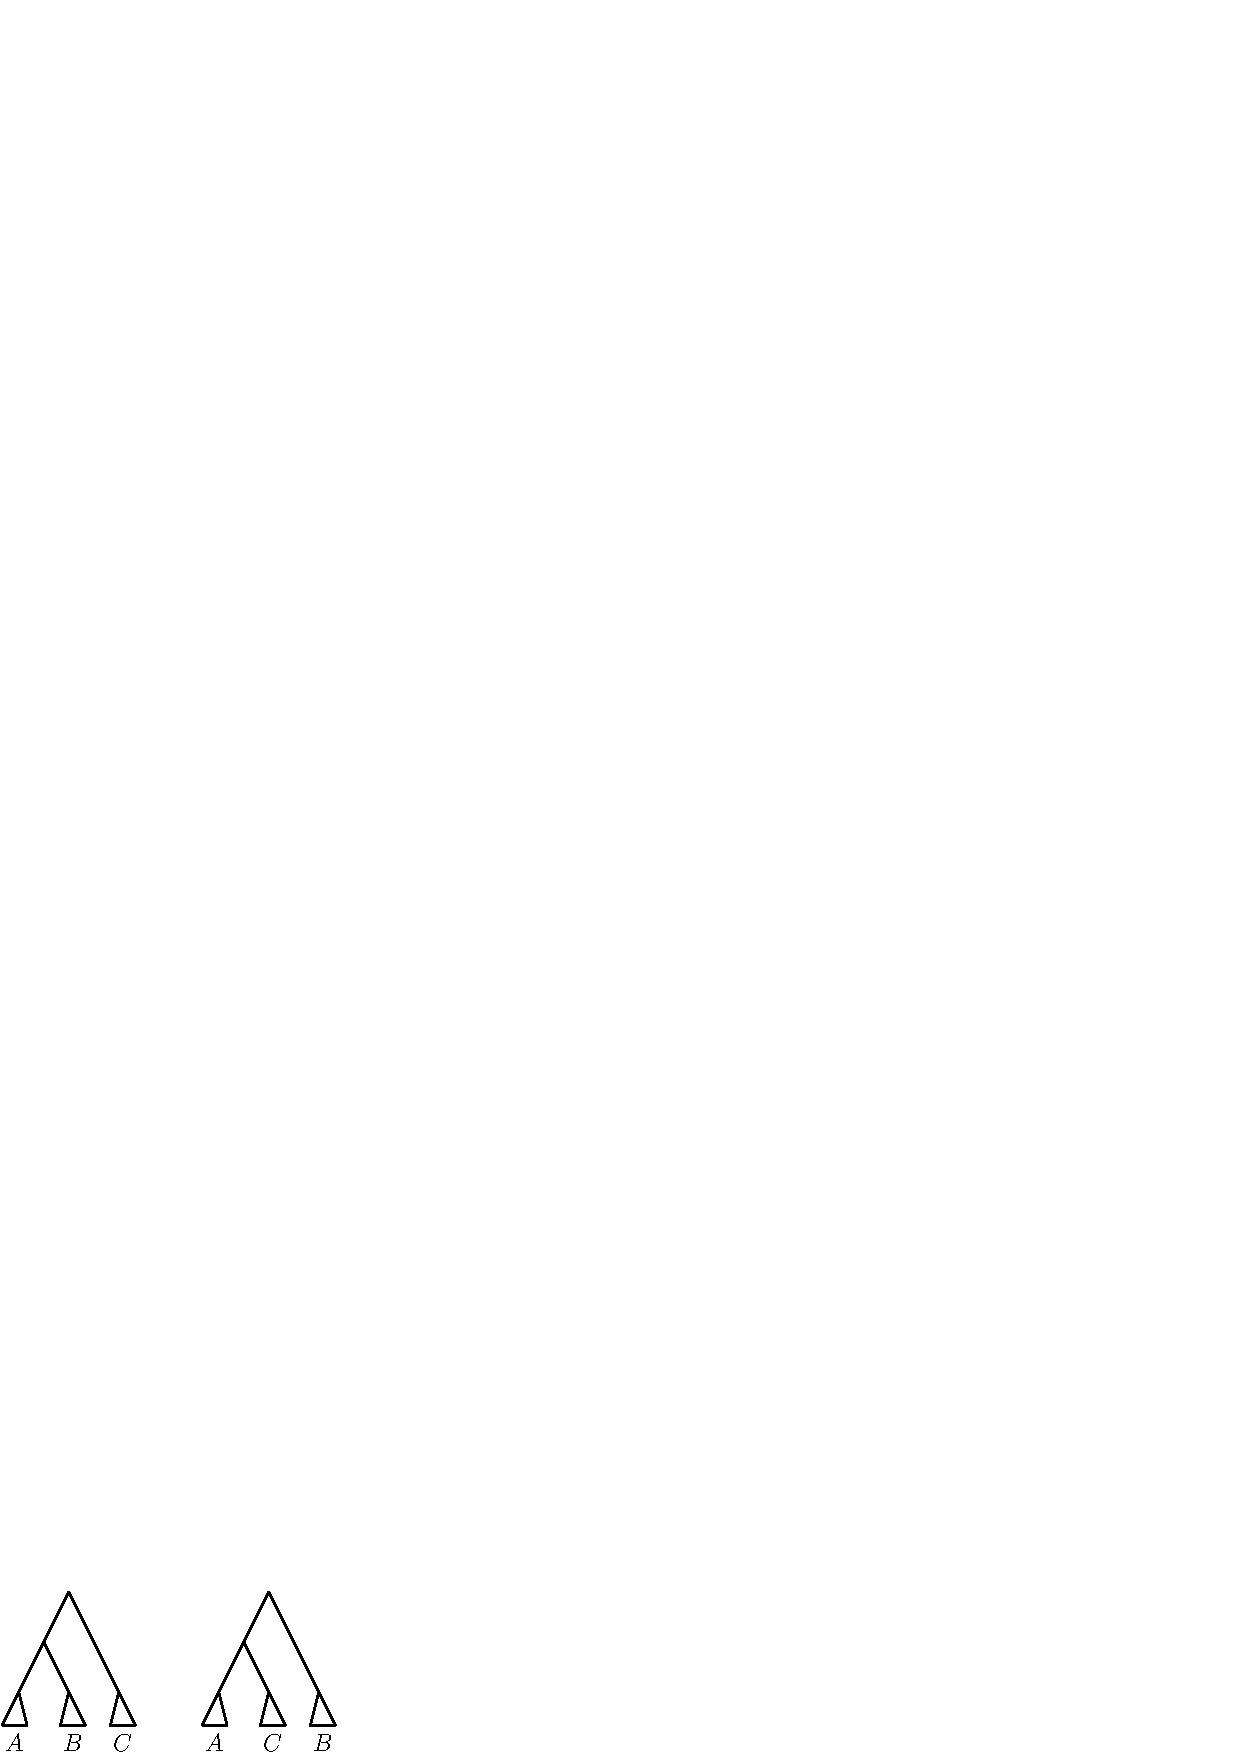
\includegraphics[width=0.4\textwidth]{NNI_move}
\vspace{12pt}
\caption{$\nni$ move}
\label{fig:nni_move}
\end{figure}

\endproof

\begin{theorem}
    Let $T,R$ be trees and $p = \findpath(T,R)$ the path from $T$ to $R$ computed by $\findpath$.
    Let $d_{FP}(T,R)$ denote the $\findpath$ distance from $T$ to $R$, that is the length of $p$.
    For all $T' \in N_1(T)$ it is $d_{FP}(T',R) \geq d_{FP}(T,R) - 1$, where $N_1(T)$ is the one-neighbourhood of $T$.
\end{theorem}

\proof

Let $p$ be a path from $T$ to $R$ computed by $\findpath$ and let $T' \in N_1(T)$ be an $\rnni$ neighbour of $T$.
With $p'$ we denote the path that $\findpath$ computes from $T'$ to $R$.

We assume that $T$ and $T'$ are the first trees on $p$ and $p'$, respectively, where a move is made that is changing one of the intervals incident to the interval $(v,w)$ (where $v$ is the node closer to the root) on which the $\rnni$ move between $T$ and $T'$ is made.
\todo{introduce notion of interval}
All moves on $p$ before this tree $T$ happen exactly the same way on $p'$ before $T'$.
Specifically, all clusters, except for the two induced by $v$ and $w$, in the cluster representations of the all trees on this first part of $p$ and $p'$ are equal.
It follows that the $\rnni$ move between the start trees of $p$ and $p'$ is the same as the move between $T$ and $T'$ as described here.
Let us consider the different possible moves that effect $v$ or $w$ on $p$ and compare them to moves that happen on $p'$.
Note that $p$ is a tree that is computed by $\findpath$ and therefore, there is a cluster $C_k$ whose most recent common ancestor is moves down by the $\rnni$ move following $T$ on $p$.

At first we consider the case that there is an $\nni$ move between $T'$ and $T$ as illustrated in the top of Figure~\ref{fig:thm_fp_nni1}.
We furthermore distinguish the different types of moves that are possible on $(v,w)$ and on the two incident intervals.

\begin{enumerate}
    \item $\nni$ moves on $e$

    If this $\nni$ move results in $T'$, it is $d_{FP}(T',R) = d_{FP}(T,R) - 1$.
    Otherwise the $\nni$ neighbour of $T$ resulting from this move is the tree on $p'$ following $T'$ as well, meaning that the remaining part of $p$ and $p'$ coincide, and it follows $d_{FP}(T',R) = d_{FP}(T,R)$.
    This is true as the $\mrca$ that is moved down by $\findpath$ on this move must contain taxa of $B$ and $C$ as depicted in Figure~\ref{fig:thm_fp_nni1}, and so this same $\mrca$ is moved down on $p'$ the same way.

    \begin{figure}[!hbt]
    \centering
    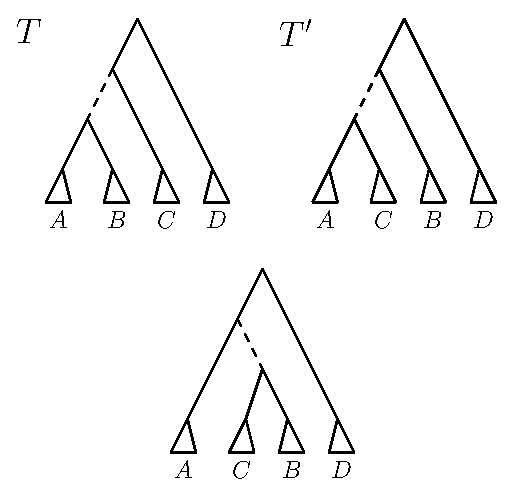
\includegraphics[width=0.4\textwidth]{thm_fp_nni1}
    \vspace{12pt}
    \caption{$\nni$ move between $T$ and $T'$ on the dashed edge and the third $\rnni$ resulting from a move on that edge.}
    \label{fig:thm_fp_nni1}
    \end{figure}

    \item $\nni$ moves on edge $f$ above $e$

    Notice that this is only possible if the interval above $e$ is an edge.
    As it is depicted in the top of Figure~\ref{fig:thm_fp_nni2a}, there are two $\nni$ moves on this edge.
    We denote the subtrees that are children of $v$ and $w$ according to the labels in that figure.

    \begin{figure}[!hbt]
    \centering
        \begin{minipage}{.45\textwidth}
            \centering
            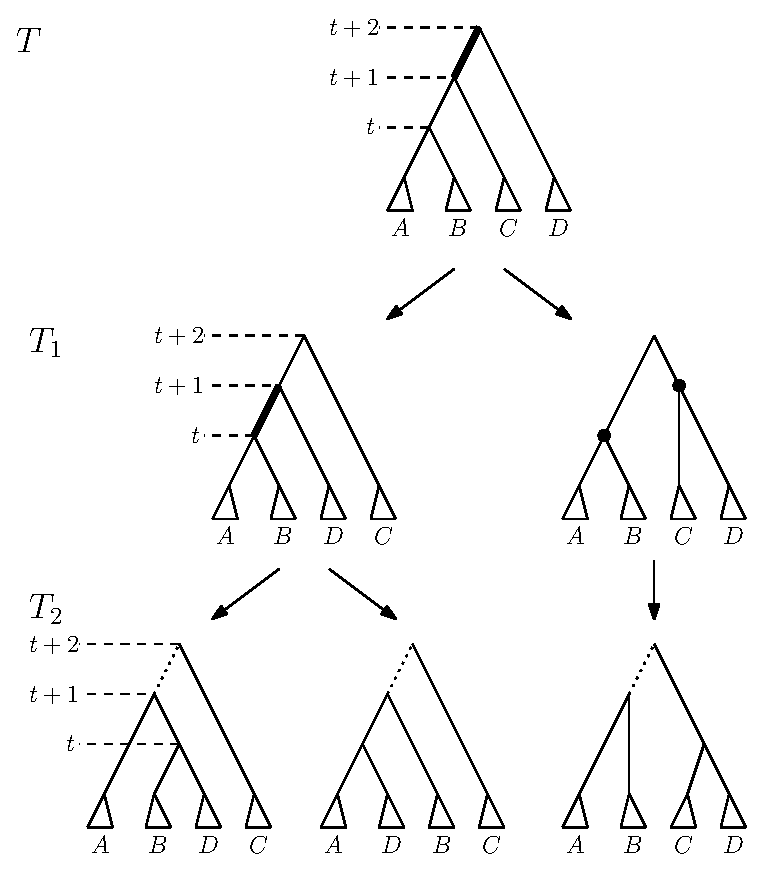
\includegraphics[width=0.9\linewidth]{thm_fp_nni2a.eps}
            \vspace{12pt}
            \label{fig:thm_fp_nni2a}
            \caption{$\nni$ moves possible on edge $f$, the dashed edge in $T$.}
        \end{minipage}
        \begin{minipage}{0.45\textwidth}
            \centering
            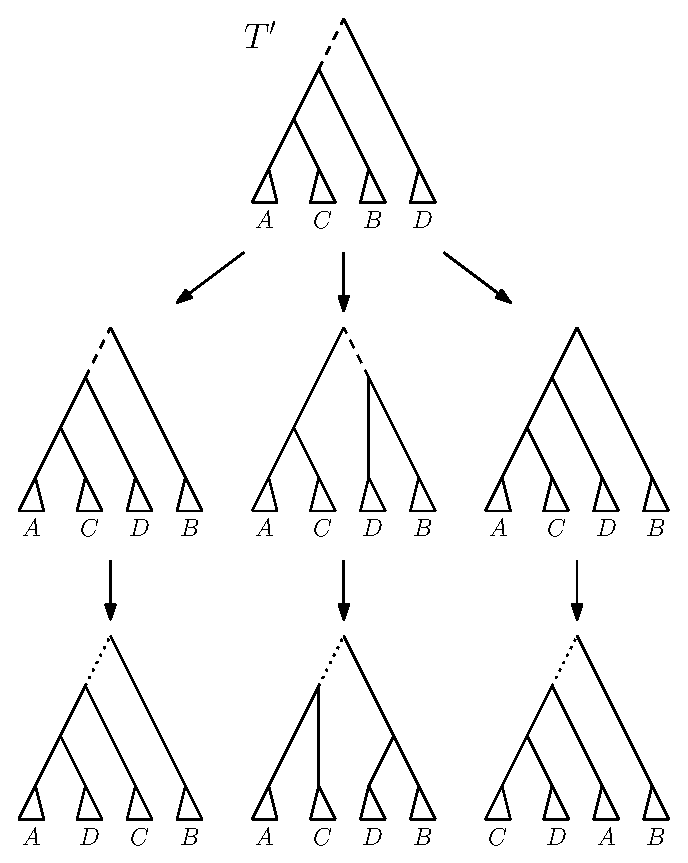
\includegraphics[width=0.9\linewidth]{thm_fp_nni2b.eps}
            \vspace{12pt}
            \label{fig:thm_fp_nni2b}
            \caption{$\nni$ moves possible on edge $f$, the dashed edge in $T$.}
        \end{minipage}
    \end{figure}

    We are considering the moves on $T$ as they are depicted in Figure~\ref{fig:thm_fp_nni2a} where we assume that $A, B, C$, and $D$ are clusters in $T$.

    If the $\nni$ move on $f$ results in the tree at the top left of Figure~\ref{fig:thm_fp_nni2a}, the cluster $C_k$ that is being moved down by $\findpath$ is either a subset of $A \cup B \cup D$, $A \cup D$ or $B \cup D$.

    \begin{enumerate}
        \item
            If $C_k \subseteq A \cup B \cup D$, the subtree containing $A \cup B$ in $T$ is the same in $R$, by the nature of $\findpath$.
            It follows that on $p'$ there is a move that moves the most recent common ancestor of $A \cup B$ down right before $C_k$ is being considered.
            It follows that on $p'$ the tree following $T'$ is $T$, resulting in $d_{FP}(T',R) = d_{FP}(T,R) + 1$.
        \item
            If $C_k \subseteq A \cup D$, the move following $T$ on $p$ moves $(C_k)_T$ further down, resulting in the tree in the bottom left of Figure~\ref{fig:thm_fp_nni2a}.
            As the same most recent common ancestor $(C_k)_{T'} \subseteq A \cup D$ moves down on $p'$, the moves that happen there starting at $T'$ are the one depicted on the left of Figure~\ref{fig:thm_fp_nni2b}.
            Comparing the trees on $p$ and $p'$ after these two moves following $T$ and $T'$, respectively, shows that we are again at a stage where two trees on these paths that only differ in one edge, meaning that we can now consider these as $T$ and $T'$ and consider the next move changing the interval distinguishing these two.
        \item
            If $C_k \subseteq B \cup D$, the two $\rnni$ moves following $T$ and $T'$ on $p$ and $p'$, respectively, end up in the trees depicted in the middle tree at the bottom of Figures~\ref{fig:thm_fp_nni2a} and \ref{fig:thm_fp_nni2b}.
            As in the previous case, these trees coincide in all but one interval and we can consider these trees as our new $T$ and $T'$.
    \end{enumerate}

    If the $\nni$ move on $f$ results in the tree on the top left of Figure~\ref{fig:thm_fp_nni2a}, it is $C_k \subseteq C \cup D$.
    If $(C_k)_T$ does not move further down on $p$, it follows that $A \cup B$ is a cluster in $R$ and that before $C_k$ is considered on $p'$, $(A \cup B)_{T'}$ moves down by one $\rnni$ move.
    This result in the tree $T$ on $p'$ right after $T'$ and it follows $d_{FP}(T',R) = d_{FP}(T,R) + 1$.
    If on the other side the rank of $(C_k)_T$ decreases further on $p$, the next move is a rank swap as depicted in the bottom right of Figure~\ref{fig:thm_fp_nni2a}.
    The moves on $p'$ that decreases the rank of $(C_k)_{T'}$ where $C_k \subseteq C \cup D$ are depicted on the right of Figure~\ref{fig:thm_fp_nni2b}.
    As above, the two trees resulting from the two moves following $T$ and $T'$ on $p$ and $p'$, respectively, coincide by all but one interval.
    Therefore, we can go back to the beginning and assume that these trees are $T$ and $T'$ now.

    \item rank move on interval $f$ above $(v,w)$

    Notice that this is only possible if the interval above $e$ is a rank interval.
    If after this rank swap increasing the rank of $v$ there is another rank swap increasing the rank of $w$, the same rank swaps happen on $p'$ and the trees after these two moves on $p$ and $p'$ coincide in all but one interval again, and we can consider them as $T$ and $T'$ now.
    If on the other side there is no such rank swap, then the cluster induced by $w$ is a cluster in $R$ as well.
    In this case, the tree following $T'$ on $p$ is $T$ as it results from building this cluster in $T'$, which happens right before the cluster $C_k$ is being considered on $p'$.
    This results in $d_{FP}(T',R) = d_{FP}(T,R) + 1$.

    \item moves on interval $g$ below $e$

    If there is a move on $g$, $C_k$ is a subset of $A \cup B$, following the notions of the trees in the top of Figure~\ref{fig:thm_fp_nni1}.
    In this case, the move following $T'$ on $p'$ moves $(C_k)_{T'}$ down by an $\nni$ move that transforms $T'$ into $T$ and it follows $d_{FP}(T',R) = d_{FP}(T,R) + 1$.

\end{enumerate}

% Let $p$ be the path computed by $\findpath(T,R)$ and let $T_0, \ldots, T_{n-1}$ be trees on $p$ such that $T_i$ is the tree after iteration $i$ of the algorithm, and $T_0 := T$.
% Define
% \[
% s(T, R) = \sum\limits_{i=1}^{n-1} (\rank((C_i)_{T_{i-1}}) - i)
% \]
% where $\rank(S)_T$ is the rank of the most recent common ancestor of cluster $S$ in tree $T$.
% Note that an inductive argument implies that it is enough to show that $s(T', R) \geq s(T, R) - 1$ for all $T' \in N_1(T)$.
% This means that there is no tree $T' \in N_1(T)$ that is more than one $\rnni$ move closer to $R$ than $T$.
%
% For proving that $s(T', R) \geq s(T, R) - 1$ for all $T' \in N_1(T)$, we distinguish all possible $\rnni$ moves between $T' \in N_1(T)$ and $T$.
%
% \begin{enumerate}
%     \item It is $\rank((C_i)_{T}) = \rank((C_i)_{T'})$ for all $i = 1, \ldots, n-1$
%     \item It is $\rank((C_i)_{T}) \neq \rank((C_i)_{T'})$ for some $i = 1, \ldots, n-1$
% \end{enumerate}
%
% %TODO: prove this. In both cases  a proof via induction might work, basis should be trivial, step similar to proof for 2 clades!?

\endproof

\begin{lemma}
Let $T$ and $R$ be $\rnni$ trees such that $\findpath(T, R)$ terminates after two iterations and returns a path $p$ of length $\ell$.
Then $\ell = d(T, R)$.
\end{lemma}

\proof
Case 1: $R = [\{1, 2\}, \{3, 4\}, \ldots]$.

Let $T'$ be the running tree after the first iteration of $\findpath(T, R)$.
Define
\[
s(T, R) = (\rank(\{1,2\})_T - 1) + (\rank(\{3,4\})_{T'} - 2)
\]
where $\rank(S)_T$ is the rank of the most recent common ancestor of cluster $S$ in tree $T$.
Note that an inductive argument implies that it is enough to show that $s(T_1, R) \geq s(T, R) - 1$ for all $T_1 \in N_1(T)$.
This means that there is no tree $T_1 \in N_1(T)$ that is more than one $\rnni$ move closer to $R$ than $T$.

For the following it is important to notice that the following holds for the path $p$ computed by $\findpath(T,R)$.
If $\mrca_T(\{1,2\}) > \mrca_T(\{3,4\})$, then there is no tree on $p$ where $\mrca(\{1,2\}) = \mrca(\{3,4\})$.

If this was possible on $p$, it could only result from an $\nni$ move that moves $\mrca(\{1,2\})$ down, and not from a rank swap.
An $\nni$ move that moves $\mrca(\{1,2\})$ down exchanges two subtrees, one of them containing taxon $1$ or $2$, the other one none of the two.
Let us call these are the subtrees $B$ and $C$ of Figure~\ref{fig:nni_move}, and without loss of generality assume that $1 \in A$ and $2 \in B$.
If after this move it is $\mrca(\{1,2\}) = \mrca(\{3,4\})$, then one of the taxa $3,4$ is in $A$ and the other one in $C$.
But then it must have been $\mrca(\{1,2\}) = \mrca(\{3,4\})$ in the tree just before this $\nni$ move already.
Therefore, it cannot be $\mrca(\{1,2\}) = \mrca(\{3,4\})$ on a tree on $p$, if it is $\mrca_T(\{1,2\}) \neq \mrca_T(\{3,4\})$ in the start tree $T$.


\begin{figure}[H]
\centering
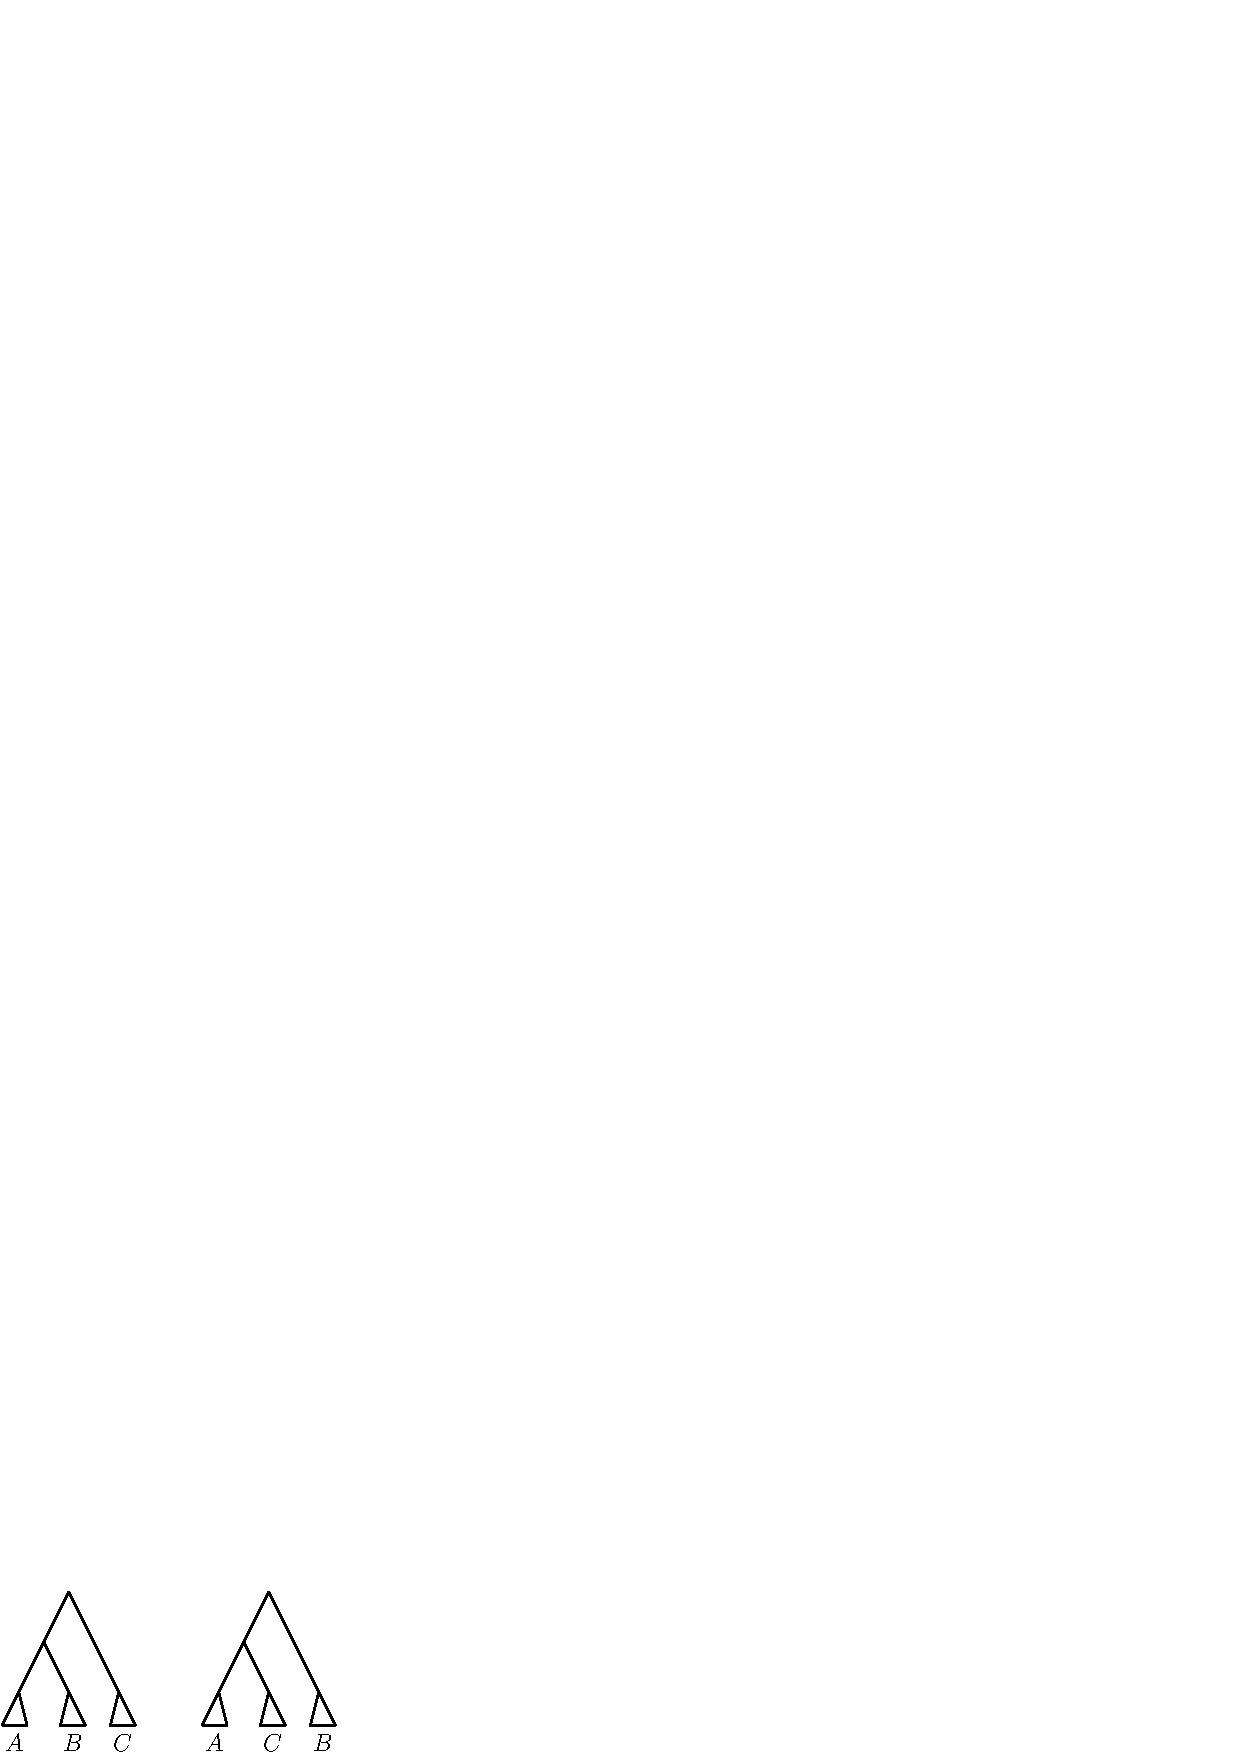
\includegraphics[width=0.4\textwidth]{NNI_move}
\vspace{12pt}
\caption{$\nni$ move}
\label{fig:nni_move}
\end{figure}

So let now $T_1 \in N_1(T)$ and let $T''$ be the tree after the first iteration of $\findpath(T_1,R)$. We will distinguish different possible $\rnni$ moves between $T$ and $T_1$ and consider how the path $\findpath(T_1,R)$ changes compared to $\findpath(T,R)$.

\begin{enumerate}

    \item The $\rnni$ move between $T$ and $T_1$ does not change the rank of $\mrca(\{1,2\})$ or $\mrca(\{3,4\})$

    It is obvious that $\rank(\{1,2\})_{T_1} = \rank(\{1,2\})_{T}$ as well as $\rank(\{3,4\})_{T''} = \rank(\{3,4\})_{T'}$, as the move between $T$ and $T_1$ does not have an effect of the ranks of these most recent common ancestors in $T$ or $T'$.
    Therefore, it is $s(T, R) = s(T_1,R)$.

    \item The $\rnni$ move between $T$ and $T_1$ changes $\rank(\mrca(\{1,2\}))$, which is not equal to $\rank(\mrca(\{3,4\}))$

    If this $\rnni$ move increases the rank of $\mrca(\{1,2\})$, the first move on $\findpath(T_1,R)$ will decrease the rank of this most recent common ancestor and results in the tree $T$, which gives us $\rank(\{1,2\})_{T_1} = \rank(\{1,2\})_{T} - 1$.
    If otherwise the rank of $\mrca(\{1,2\})$ decreases by the $\rnni$ move from $T$ to $T_1$, it is $\rank(\{1,2\})_{T_1} = \rank(\{1,2\})_T - 1$.
    However, the rank of $\mrca(\{3,4\})$ is the same in $T'$ and $T''$, no matter whether $\rank(\mrca(\{1,2\}))$ decreases or increases.
    The only point at which $\rank(\mrca(\{3,4\}))$ could change on the path is if there is an exchange of ranks of $\mrca(\{1,2\})$ and $\mrca(\{3,4\})$ in the first iteration of $\findpath(T_1,R)$.
    But this just happens if and only if the same exchange of ranks happens on $\findpath(T,R)$, hence it is $s(T_1,R) \geq s(T,R) - 1$ in this case.

    \item The $\rnni$ move between $T$ and $T_1$ changes $\rank(\mrca(\{1,2\}))$, which is equal to $\rank(\mrca(\{3,4\}))$

    If the move from $T$ to $T_1$ increases the rank of $\mrca(\{1,2\})$, the first tree on $\findpath(T_1,R)$ is $T$, as there always is exactly one $\rnni$ move that moves $\mrca(\{1,2\})$ down, which in this case is the move that moves both $\mrca(\{1,2\})$ and $\mrca(\{3,4\})$ down.
    Then it is $\rank(\{1,2\})_{T_1} = \rank(\{1,2\})_{T} + 1$ and $\rank(\{3,4\})_{T''} = \rank(\{3,4\})_{T'}$ and therefore $s(T_1,R) = s(T,R) + 1$ in this case.
    And if the rank of $\mrca(\{1,2\})$ decreases from $T$ to $T_1$, $T_1$ is the first tree on $\findpath(T,R)$, which results in $s(T_1,R) = s(T,R) - 1$.

    \item The $\rnni$ move between $T$ and $T_1$ changes $\rank(\mrca(\{3,4\}))$, which is not equal to $\rank(\mrca(\{1,2\}))$

    In this case it obviously is $\rank(\{1,2\})_{T_1} = \rank(\{1,2\})_{T}$.
    Also, the rank of $\mrca(\{3,4\})$ changes on the path from $T_1$ to $T''$ if and only if it does on the path from $T$ to $T'$.
    Note that this rank can change by at most one when this most recent common ancestor exchanges ranks with $\mrca(\{1,2\})$.
    Therefore, it is either $\rank(\{3,4\})_{T''} = \rank(\{3,4\})_{T'} + 1$ or $\rank(\{3,4\})_{T''} = \rank(\{3,4\})_{T'} - 1$, depending on whether the move between $T$ and $T_1$ increases or decreases the rank of $\mrca(\{3,4\})$.
    In either case it is $s(T_1,R) \geq s(T,R) - 1$
\end{enumerate}

We can conclude that in any case it is $s(T_1,R) \geq s(T,R) - 1$.


Case 2: $R = [\{1, 2\}, \{1, 2, 3\}, \ldots]$.

The same as case 1, the only difference is that $\mrca(\{1,2\}) > \mrca(\{1,2,3\})$ is not possible.
%TODO Check whether this really is true!
\endproof
\end{document}
